% !TeX encoding = UTF-8
% !TeX program = xelatex
% !TeX spellcheck = fr
% !TeX root = tm_astro_main.tex


\chapter{L'E-ELT}\label{4}

L'European Extremely Large Telescope est un télescope optique actuellement en cours de construction qui est développé par l'European Southern Observatory (ESO) depuis 2005. Comme son nom l'indique, il fait partie de la catégorie des Extremely Large Telescope (ELT). Cette classe contient tout les télescopes optiques possédant un miroir primaire de diamètre supérieur à 20 mètres. Il existe à ce jour 3 ELT en construction (nous en reparlerons dans la section \ref{4.3}); leur mise en service respective est prévue entre 2024 et 2027. L'ELT qui nous intéresse dans ce travail, l'E-ELT, possède, avec ses 39.3 mètres, le plus grand miroir de la catégorie des télescopes géants et par extension le plus grand télescope optique jamais construit. Son lieu de construction à 3060 mètres d'altitude se situe à Cerro Armazones dans le désert d'Atacama au Chili. La taille de son miroir primaire ainsi que la faculté d'observer dans le spectre visible et l'infrarouge lui permettront d'éclairer de nombreuses zones d'ombre concernant des sujets tels que: les exoplanètes, la population stellaire des galaxies ou encore le cycle de vie des étoiles enrichissant le milieu interstellaire (§\ref{5}).

\begin{figure}[H]
	\centering
	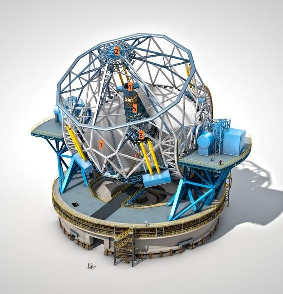
\includegraphics[scale=1.35]{images/e-elt_i}
	\caption[Vue d'artiste de l'E-ELT avec les 5 miroirs primaires \label{Fig. 4.1}]{Vue d'artiste de l'E-ELT avec les 5 miroirs primaires}
	\addloflink{https://fis-landschaft.de/universum/elt/}
	\label{Fig. 4.1}
\end{figure}

\section{Les raisons et les technologies nécessaires à la construction de l'E-ELT}\label{4.1}

Au fur et à mesure que la recherche scientifique en astronomie progresse, des télescopes de plus en plus performants sont nécessaires. Pour cela, il existe plusieurs manières d'accroître la qualité d'un télescope. L'une de ces manières consiste à augmenter la quantité de lumière collectée en grossissant le diamètre de l'instrument, cela permet d'augmenter la quantité de détails observés. Une autre des solutions réside dans l'augmentation de la qualité des différents instruments traitant l'image créée par le télescope. A ce jour, ces instruments ont atteint une qualité quasi-parfaite, donc la seule solution pour augmenter les performances des télescopes est d'en construire des plus gros. Cependant, il n'est pas si simple de fabriquer un miroir de 39 mètres tout en évitant des aspérités plus grandes que 150 $\mu m$ lors du polissage, de plus les contraintes liées au poids du miroir rendraient quasi-impossible la fabrication de celui-ci. Pour contrer ce problème, le miroir de l'E-ELT ne sera pas construit en une seule pièce, il utilisera plutôt la technique du miroir segmenté. Cette technique, utilisée pour la première fois en 1979 avec le Multiple Mirror Telescope, consiste à remplacer un grand miroir par un grand nombre de plus petits miroirs assemblés les uns avec les autres. Ainsi, l'E-ELT sera composé de 798 miroirs hexagonaux de 1.44 mètres de côté, qui constitueront au total 5 grands miroirs primaires (Fig. \ref{Fig. 4.1}). L'E-ELT bénéficie encore d'une technologie récente permettant d'énormes progrès à l'observation terrestre, l'optique adaptative. Cette technologie a pour but de corriger les perturbations atmosphériques\footnotemark[1] en utilisant 6 lasers qui l'analyseront en permanence. Ces-derniers seront couplés à un système de vérins qui pourront déformer les miroirs 4 et 5 pour compenser les turbulences atmosphériques jusqu'à 1000 fois par seconde.

\section{Les instruments}\label{4.2}

De nombreux projets pour instrumenter l'E-ELT ont été proposés à l'ESO. Cependant, pour des raisons budgétaires et structurelles l'organisation a du faire une sélection parmi toutes ces propositions. La phase de sélection a approuvé en 2015 la construction de 4 instruments pour équiper le télescope géant:

\begin{itemize}
	
	\item MICADO: La Multi-AO Imaging CamerA for Deep Observations est une caméra infrarouge ainsi qu'un spectographe\footnotemark[2] qui travaillera en tandem avec le deuxième instrument sélectionné (MAORY, qui lui fournira une optique adaptative). Ses principaux buts scientifiques sont l'étude de l'environnement et de la structure des galaxies à grand décalage vers le rouge\footnotemark[3] et le mouvement des étoiles proches du trou noir se trouvant au centre de notre galaxie. 
	
	\item MAORY: La Multi-conjugate Adaptive Optics RelaY est un système d'optique adaptative qui sera utilisé pour augmenter les performances de MICADO en compensant les turbulences de l'atmosphère.
	
	\item HARMONI: Le High Angular Resolution Monolithic Optical and Near-infrared Integral field spectrograph est un spectrographe\footnotemark[2] pouvant opérer à la fois dans le spectre visible et dans le proche infrarouge. L'étude des exoplanètes ainsi que la formation et l'évolution des galaxies à grand décalage vers le rouge\footnotemark[3] représentent ses principaux domaines d'études.
	
	\item METIS: The Mid-infrared ELT Imager and Spectrograph est un spectrographe\footnotemark[2] qui a aussi pour domaine d'étude les exoplanètes. Cependant, il étudiera aussi des sujets tels que l'atmosphère marsienne ou encore les rayons gammas.
	
\end{itemize}

Tout ces instruments sont développées par des consortiums d'universités ou centres de recherches européens. Leur mise en service est prévue pour 2025.
	
\vfill

\footnotetext[1]{Les perturbations atmosphériques se caractérisent par une image turbulente et un peu floue.}
\footnotetext[2]{Un spectrographe est un instrument qui permet de séparer et d'enregistrer les différentes couleurs composant une source lumineuse.}	
\footnotetext[3]{Le décalage vers le rouge représente le fait qu'un signal lumineux émis dans le spectre visible par un objet est décalé dans l'infrarouge par effet Doppler; cela a pour signification que l'objet observé s'éloigne de nous à grande vitesse.}

\newpage

\section{Comparaison avec d'autres télescopes}\label{4.3}

A ce jour, le télescope optique terrestre le plus performant est le Very Large Telescope (VLT).Grâce aux plus récents systèmes d'optique adaptative le VLT dépasse les performances du télescope spatial Hubble dans certains domaines. Le Very Large Telescope est composé de 4 miroirs primaires de 8.2 mètres, qui peuvent être utilisés seuls ou bien reliés par interférométrie.  A titre de comparaison, l'E-ELT pourra collecter jusqu'à 15 fois plus de lumière que le VLT. Comme nous en avons parlé au début de ce chapitre, l'E-ELT fait partie de la classe des Extremely Large Telescope (ELT). Les 2 autres télescopes faisant partie de cette catégorie sont le Télescope de Trente Mètres (TMT) avec, comme son nom l'indique, un miroir primaire de 30 mètres et le Télescope géant Magellan (GMT) constitué de 7 miroirs de 8.4 mètres qui forment un miroir de 21.4 mètres de diamètre. Ces deux instruments américains sont aussi plus performants que le VLT mais restent inférieurs en terme de surface collectrice et de diamètre par rapport à l'E-ELT.  

\begin{figure}[H]
	\centering
	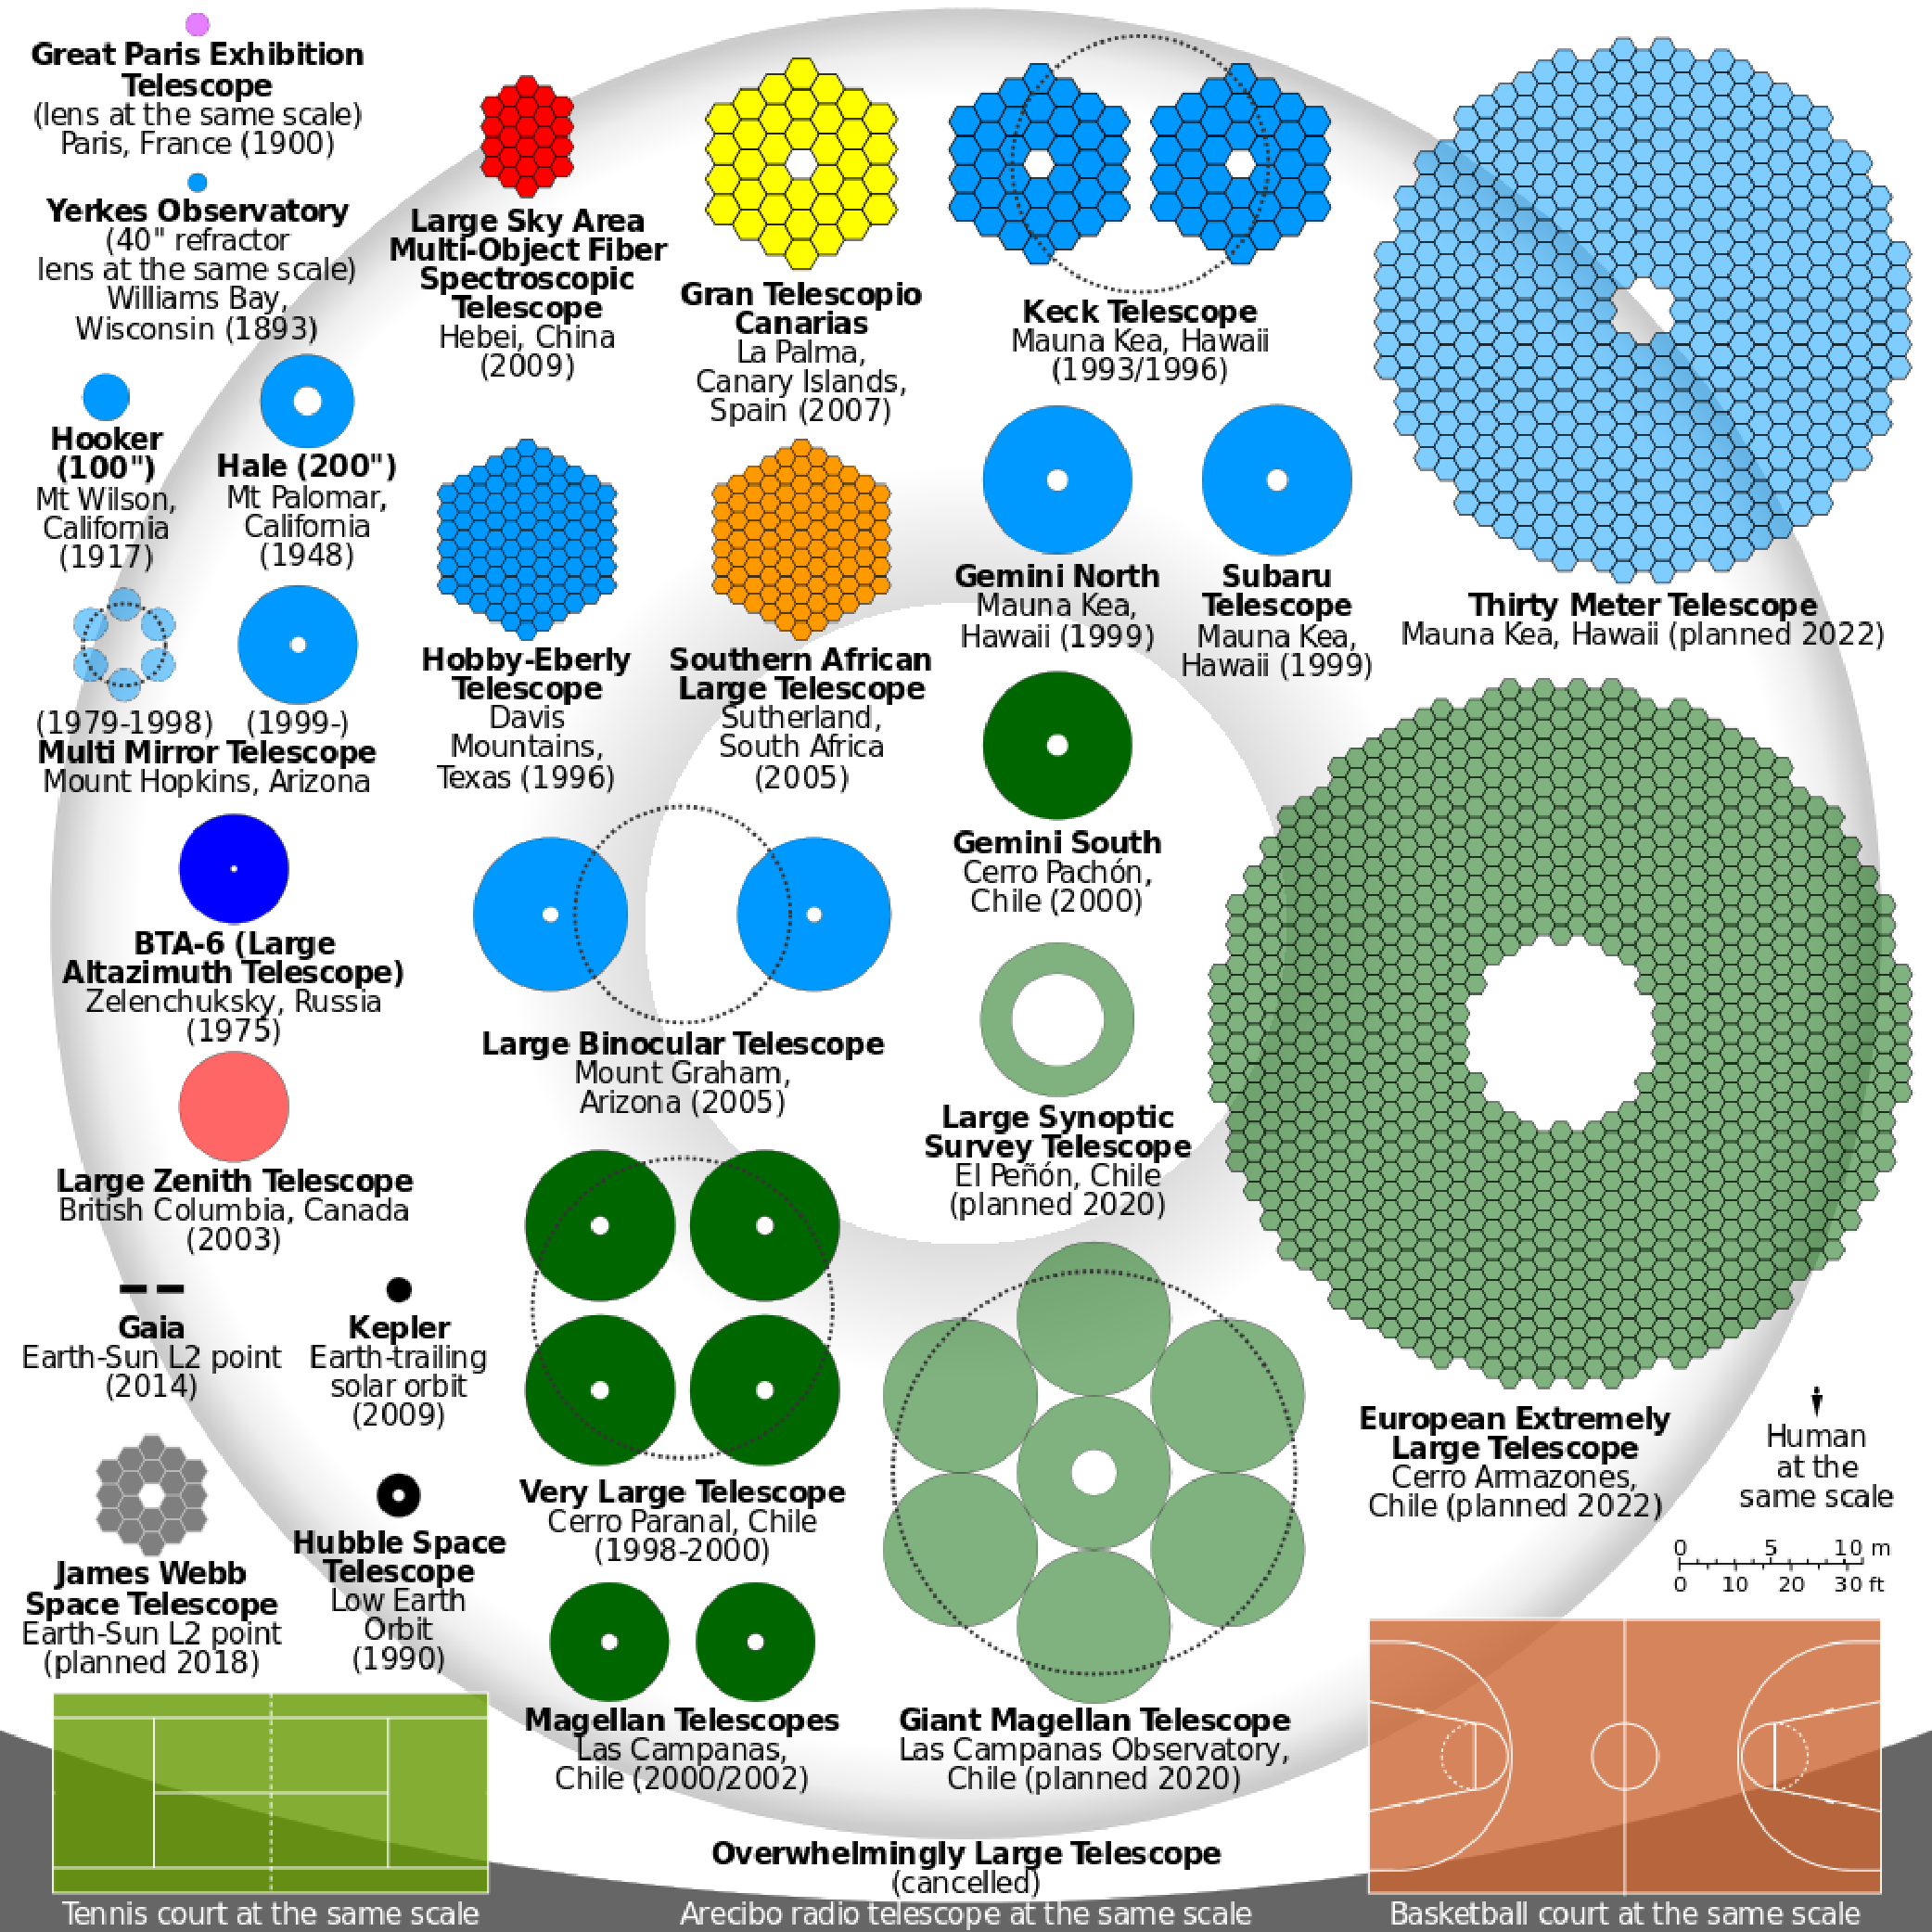
\includegraphics[scale=0.2]{images/comp_tscp}
	\caption[Comparaison des miroirs primaires de plusieurs télescopes]{Comparaison des miroirs primaires de plusieurs télescopes}
	\addloflink{https://en.wikipedia.org/wiki/Segmented_mirror}
	\label{Fig. 4.2}
\end{figure}

Pour finir, il convient de comparer le plus grand projet de télescope optique terrestre, l'E-ELT avec son homologue spatial, Le James Webb Space Telescope (JWST). Cette comparaison a du sens car ils possèdent tout les deux des points communs au niveau de leur objectifs scientifiques (étude des premières galaxies, formation de système planétaire). Tout d'abord, le miroir du JWST mesure 6.5 mètres de diamètre, il possède ainsi une surface collectrice environ 36 fois inférieure à celle de l'E-ELT. Cependant, ce déficit de taille est largement compensé par le fait que le JWST se trouvera hors de notre atmosphère et s'affranchira ainsi de toute perturbation atmosphérique. Comme les rayons infrarouges sont en partie filtrés par l'atmosphère, l'E-ELT se focalisera sur le spectre visible et le proche infrarouge; le JWST, qui s'affranchit donc de cette absorption, ne sera pas équipé pour observer le spectre visible, il fera uniquement des observations dans l'infrarouge. L'un des majeur problème des télescopes spatiaux en général est leur maintenance; le James Webb se situera à une distance de 1.5 millions de kilomètres de la Terre, ce qui rend impossible toute mission de maintenance. Au niveau budgétaire, c'est l'E-ELT qui l'emporte très clairement avec un coût de fabrication quasiment 10 fois inférieur à celui du JWST (1.2 milliards de dollars pour l'E-ELT et environ 10 milliards de dollars pour le JWST). En conclusion, il est difficile de les départager, chacun possède ses avantages et ses inconvénients; néanmoins, ce qui est sûr c'est que ces 2 télescopes représentent d'ores et déjà l'avenir de l'astronomie. 